%%%%%%%%%%%%%%%%%%%%%%%%%%%%%%%%%%%%%%%%%
% Engineering Calculation Paper
% LaTeX Template
% Version 1.0 (20/1/13)
%
% This template has been downloaded from:
% http://www.LaTeXTemplates.com
%
% Original author:
% Dmitry Volynkin (dim_voly@yahoo.com.au)
%
% License:
% CC BY-NC-SA 3.0 (http://creativecommons.org/licenses/by-nc-sa/3.0/)
%
%%%%%%%%%%%%%%%%%%%%%%%%%%%%%%%%%%%%%%%%%

%----------------------------------------------------------------------------------------
%	PACKAGES AND OTHER DOCUMENT CONFIGURATIONS
%----------------------------------------------------------------------------------------

\documentclass[10pt,a4paper]{article} % Use A4 paper with a 12pt font size - different paper sizes will require manual recalculation of page margins and border positions

\usepackage{marginnote} % Required for margin notes
\usepackage{wallpaper} % Required to set each page to have a background
\usepackage{lastpage} % Required to print the total number of pages
\usepackage[left=1.3cm,right=4.6cm,top=1.8cm,bottom=4.0cm,marginparwidth=3.4cm]{geometry} % Adjust page margins
\usepackage{amsmath} % Required for equation customization
\usepackage{amssymb} % Required to include mathematical symbols
\usepackage{xcolor} % Required to specify colors by name
\usepackage{listings}

\usepackage{fancyhdr} % Required to customize headers
\setlength{\headheight}{80pt} % Increase the size of the header to accommodate meta-information
\pagestyle{fancy}\fancyhf{} % Use the custom header specified below
\renewcommand{\headrulewidth}{0pt} % Remove the default horizontal rule under the header

\setlength{\parindent}{0cm} % Remove paragraph indentation
\newcommand{\tab}{\hspace*{2em}} % Defines a new command for some horizontal space

\newcommand\BackgroundStructure{ % Command to specify the background of each page
\setlength{\unitlength}{1mm} % Set the unit length to millimeters

\definecolor{amaranth}{rgb}{0.9, 0.17, 0.31}
\definecolor{babyblueeyes}{rgb}{0.63, 0.79, 0.95}
\definecolor{beige}{rgb}{0.96, 0.96, 0.86}
\definecolor{bittersweet}{rgb}{1.0, 0.44, 0.37}
\definecolor{black}{rgb}{0.0, 0.0, 0.0}
\definecolor{bleudefrance}{rgb}{0.19, 0.55, 0.91}
\definecolor{bostonuniversityred}{rgb}{0.8, 0.0, 0.0}
\definecolor{brightube}{rgb}{0.82, 0.62, 0.91}
\definecolor{darkseagreen}{rgb}{0.56, 0.74, 0.56}
\definecolor{lavender}{rgb}{0.9, 0.9, 0.98}
\definecolor{mayablue}{rgb}{0.45, 0.76, 0.98}
\definecolor{cadmiumgreen}{rgb}{0.0, 0.42, 0.24}
\definecolor{almond}{rgb}{0.94, 0.87, 0.8}
\definecolor{antiquewhite}{rgb}{0.98, 0.92, 0.84}
\definecolor{ashgrey}{rgb}{0.7, 0.75, 0.71}
\definecolor{babyblueeyes}{rgb}{0.63, 0.79, 0.95}
\definecolor{beige}{rgb}{0.96, 0.96, 0.86}
\definecolor{blond}{rgb}{0.98, 0.94, 0.75}
\definecolor{cream}{rgb}{1.0, 0.99, 0.82}
\definecolor{eggshell}{rgb}{0.94, 0.92, 0.84}

\setlength\fboxsep{0mm} % Adjusts the distance between the frameboxes and the borderlines
\setlength\fboxrule{0.5mm} % Increase the thickness of the border line
\put(10, 10){\fcolorbox{black}{darkseagreen!10}{\framebox(155,247){}}} % Main content box
\put(165, 10){\fcolorbox{black}{blond!10}{\framebox(37,247){}}} % Margin box
\put(10, 262){\fcolorbox{black}{amaranth!10}{\framebox(192, 25){}}} % Header box
\put(170, 263){
\includegraphics[height=23mm,keepaspectratio]{csm}} % Logo box - maximum height/width: 
}

%----------------------------------------------------------------------------------------
%	HEADER INFORMATION
%----------------------------------------------------------------------------------------

\fancyhead[L]{
\begin{tabular}{l l | l l} % The header is a table with 4 columns
\textbf{CSC447:} & Parallel Programming &  \textbf{Name:} & Samer Saber  \\ % Project name and page count
\textbf{Lab 1:}  & Pi using Pthreads &   \textbf{ID:}  & 201401460\\ % Project name and page count
\textbf{Date:}&   \today &  \textbf{Page:} & \thepage/\pageref{LastPage}  \\ % Project name and page count
\textbf{Spring 2022} & & & \\ % Version and reviewed date
\end{tabular}}


 

%&  & \textbf{Date} & 27/11/2012 \\ % Job number and last updated date


%----------------------------------------------------------------------------------------

\begin{document}

\AddToShipoutPicture{\BackgroundStructure} % Set the background of each page to that specified above in the header information section

%----------------------------------------------------------------------------------------
%	DOCUMENT CONTENT
%----------------------------------------------------------------------------------------

\subsection*{Abstract}

Making observations on each code and extracting the running time.
\section{Introduction}

Implementing all the codes and observing the results after each run to check the performance.

\section{Implementation}

1- Reproducing the serial code:

\begin{lstlisting}[language=C, caption=C Example]
#include <stdio.h>
#include <stdlib.h>
#include <time.h>

int main()
{
	int 		array_size;
	int 		counter;
	int * 		rand_arr;
	double		duration;
	clock_t		start;
	clock_t		end;

	array_size	= 10000000;
	counter		= 0;
	rand_arr	= calloc(array_size, sizeof(int));
	srand(time(NULL));
	start		= clock();

	for (int i = 0; i < array_size; i++)
    {
        rand_arr[i] = rand() % 10;
        if (rand_arr[i] == 3)
        {
            counter++;
        }
    }

	end		= clock();
	duration= ((double)(end - start) / CLOCKS_PER_SEC) * 1000;
	printf("There are %d 3s and it takes %fms", counter, duration);
	return 0;
}
\end{lstlisting}

2- Implementing data race:

\begin{lstlisting}[language=C, caption=C Example]
#include <stdio.h>
#include <stdlib.h>
#include <time.h>
#include <pthread.h>

#define MaxThreads 1000
void* count3s_thread(void* id);
pthread_t tid[MaxThreads];

int t;         /* number of threads */
int * array;
int length;
int count;

void count3s()
{
   int i;
   count = 0;
   /* Create t threads */
   for(i = 0; i < t; i++)
   {
      pthread_create(&tid[i], NULL, count3s_thread, (void*)i);
   }

   /*** wait for the threads to finish ***/
   for(i = 0; i < t; i++)
   {
      pthread_join(tid[i], NULL);
   }
}

void* count3s_thread(void* id)
{
   int i;
   /* Compute portion of the array that this thread should work on */
   int length_per_thread = length / t;
   int start = (intptr_t)id * length_per_thread;

   for(i = start; i < start+length_per_thread; i++)
   {
      if(array[i] == 3)
      {
         count++;
      }
   }
   return 0;
}


int main(int argc, char *argv[])
{
   int i;
   length = 1048576;  /*  2^20  */
   t = 40;  /*** be sure that t divides length!! ***/

   array = calloc(length, sizeof(int));

   /* initialize the array with random integers between 0 and 9 */
   srand(time(NULL));  /* seed the random number generator with current time */
   for(i = 0; i < length; i++)
   {
      array[i] = rand()%10;
   }

   clock_t start = clock();
   count3s();
   clock_t end = clock();
   double time_spent = ((double)(end - start) / CLOCKS_PER_SEC) * 1000.0;
   printf("It takes %fms\n", time_spent);

   printf("Parallel: The number of 3's is %d\n", count);

   count = 0;
   for (i = 0; i < length; i++)
      if (array[i] == 3)
         count++;
   printf("Serial: The number of 3's is %d\n", count);

   return 0;
}
\end{lstlisting}

3- Implementing data race with locks only:

\begin{lstlisting}[language=C, caption=C Example]
#include <stdio.h>
#include <stdlib.h>
#include <time.h>
#include <pthread.h>

#define MaxThreads 1000
void* count3s_thread(void* id);
pthread_t tid[MaxThreads];

int t;         /* number of threads */
int * array;
int length;
int count;

pthread_mutex_t m = PTHREAD_MUTEX_INITIALIZER;

void count3s()
{
   int i;
   count = 0;
   /* Create t threads */
   for(i = 0; i < t; i++)
   {
      pthread_create(&tid[i], NULL, count3s_thread, (void*)i);
   }

   /*** wait for the threads to finish ***/
   for(i = 0; i < t; i++)
   {
      pthread_join(tid[i], NULL);
   }
}

void* count3s_thread(void* id)
{
   int i;
   /* Compute portion of the array that this thread should work on */
   int length_per_thread = length / t;
   int start = (intptr_t)id * length_per_thread;

   for(i = start; i < start+length_per_thread; i++)
   {
      if(array[i] == 3)
      {
         pthread_mutex_lock(&m);
         count++;
         pthread_mutex_unlock(&m);
      }
   }
   return 0;
}


int main(int argc, char *argv[])
{
   int i;
   length = 1048576;  /*  2^20  */
   t = 40;  /*** be sure that t divides length!! ***/

   array = calloc(length, sizeof(int));

   /* initialize the array with random integers between 0 and 9 */
   srand(time(NULL));  /* seed the random number generator with current time */
   for(i = 0; i < length; i++)
   {
      array[i] = rand()%10;
   }

   clock_t start = clock();
   count3s();
   clock_t end = clock();
   double time_spent = ((double)(end - start) / CLOCKS_PER_SEC) * 1000.0;
   printf("It takes %fms\n", time_spent);

   printf("Parallel: The number of 3's is %d\n", count);

   count = 0;
   for (i = 0; i < length; i++)
      if (array[i] == 3)
         count++;
   printf("Serial: The number of 3's is %d\n", count);

   return 0;
}
\end{lstlisting}

4- data race with locks and padding:

\begin{lstlisting}[language=C, caption=C Example]
#include <stdio.h>
#include <stdlib.h>
#include <time.h>
#include <pthread.h>

#define MaxThreads 1000
void* count3s_thread(void* id);
pthread_t tid[MaxThreads];

int t;         /* number of threads */
int * array;
int length;
int count;

struct padded_int
{
    int value;
    char padding[60];
} private_count[MaxThreads];
pthread_mutex_t m = PTHREAD_MUTEX_INITIALIZER;

void count3s()
{
   int i;
   count = 0;
   /* Create t threads */
   for(i = 0; i < t; i++)
   {
      pthread_create(&tid[i], NULL, count3s_thread, (void*)i);
   }

   /*** wait for the threads to finish ***/
   for(i = 0; i < t; i++)
   {
      pthread_join(tid[i], NULL);
   }
}

void* count3s_thread(void* id)
{
   int i;
   /* Compute portion of the array that this thread should work on */
   int length_per_thread = length / t;
   int start = (int)id * length_per_thread;

   for(i = start; i < start+length_per_thread; i++)
   {
      if(array[i] == 3)
      {
         private_count[(int)id].value++;
      }
   }
   pthread_mutex_lock(&m);
   count += private_count[(int)id].value;
   pthread_mutex_unlock(&m);

   return 0;
}


int main(int argc, char *argv[])
{
   int i;
   length = 1048576;  /*  2^20  */
   t = 40;  /*** be sure that t divides length!! ***/

   array = calloc(length, sizeof(int));

   /* initialize the array with random integers between 0 and 9 */
   srand(time(NULL));  /* seed the random number generator with current time */
   for(i = 0; i < length; i++)
   {
      array[i] = rand()%10;
   }

   clock_t start = clock();
   count3s();
   clock_t end = clock();
   double time_spent = ((double)(end - start) / CLOCKS_PER_SEC) * 1000.0;
   printf("It takes %fms\n", time_spent);

   printf("Parallel: The number of 3's is %d\n", count);

   count = 0;
   for (i = 0; i < length; i++)
      if (array[i] == 3)
         count++;
   printf("Serial: The number of 3's is %d\n", count);

   return 0;
}
\end{lstlisting}

\section{Experimental Platform}
Windows 10, Sublime text editor and a GCC compiler

\section{Results}

no padding:

\begin{figure}
    \centering
    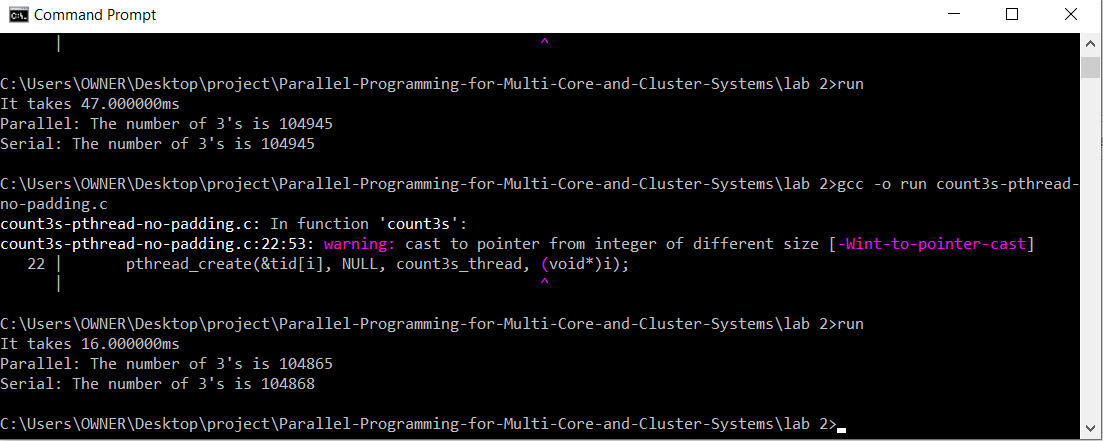
\includegraphics[width=12cm]{no-padding.png}
    \caption{A screenshot of the terminal for no padding}
    \label{fig:no padding}

no padding but locks only:

    \centering
    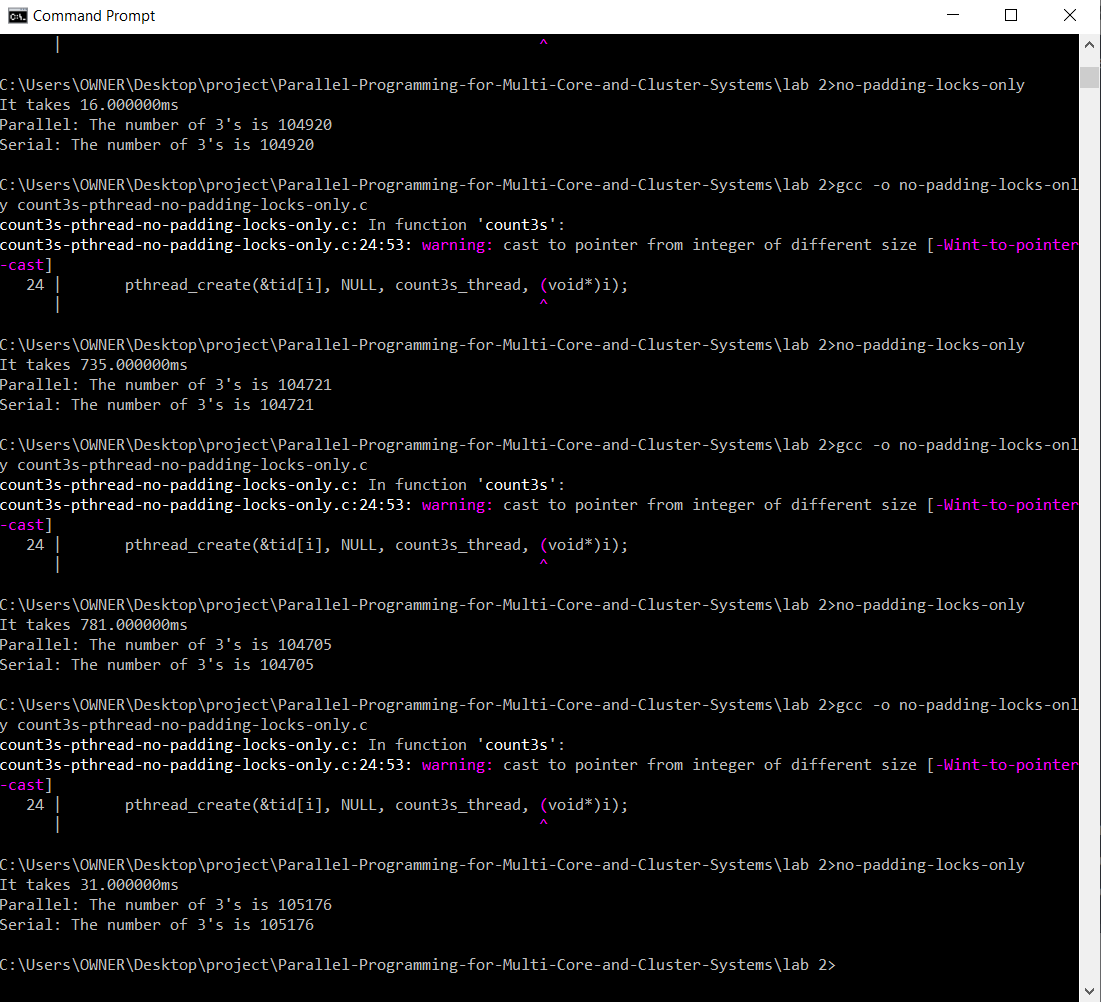
\includegraphics[width=12cm]{no-padding-locks.png}
    \caption{A screenshot of the terminal for no padding but locks only}
    \label{fig:locks}

With padding and locks:

    \centering
    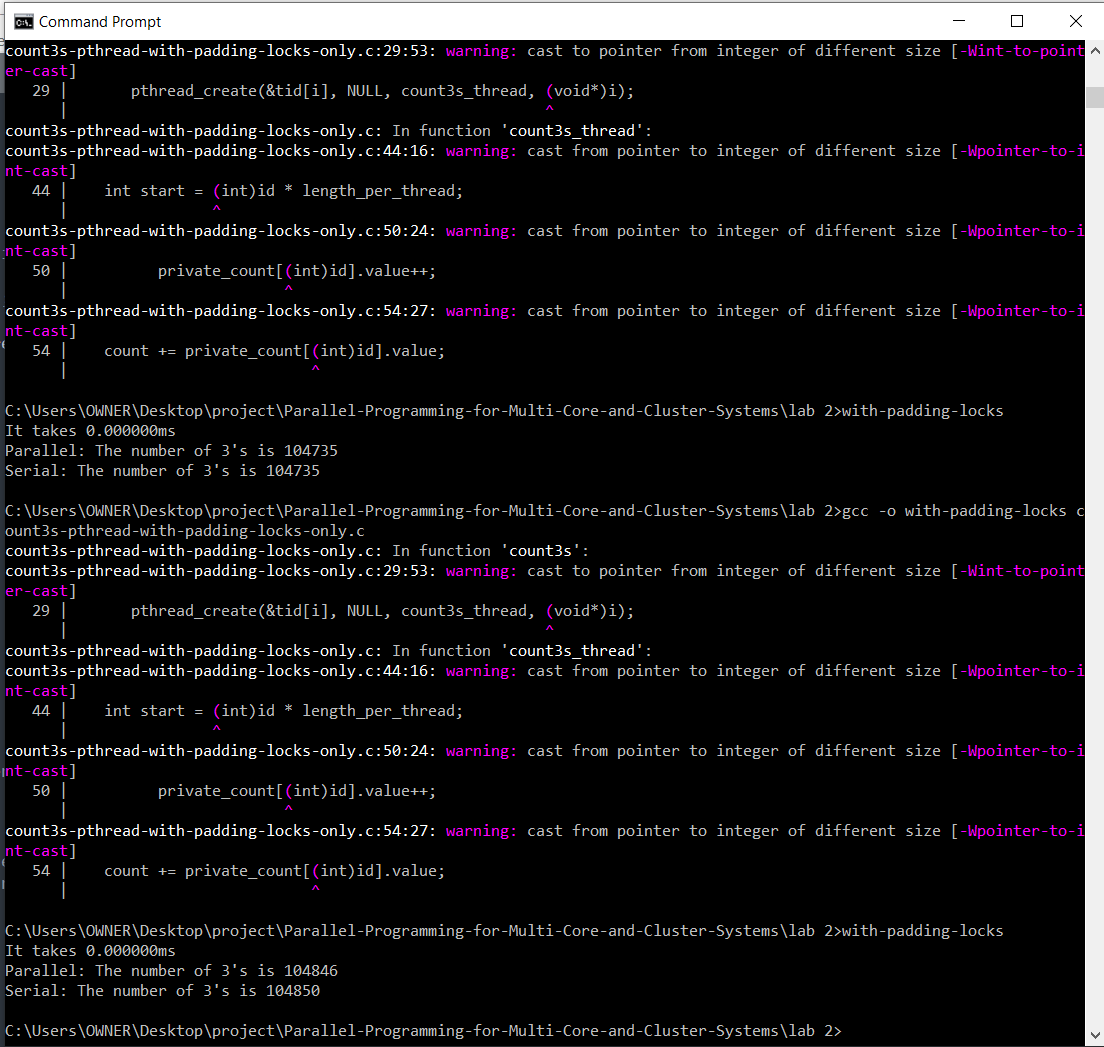
\includegraphics[width=12cm]{with-padding-lock.png}
    \caption{A screenshot of the terminal for padding and locks only}
    \label{fig:paddingLocks}
\end{figure}

\vspace{10cm}

\section{Discussion}

We notice after running the codes with different array sizes, that the bigger the array the lower the performance.
Also, locks and padding make the results more correct.
And, when the number of threads is increases the code runs faster.


\section{Conclusion}
Race conditions are hard to deal with in parallel programming

%----------------------------------------------------------------------------------------

\end{document}